\documentclass[main.tex]{subfiles}

\begin{document}

\begin{multicols}{2}

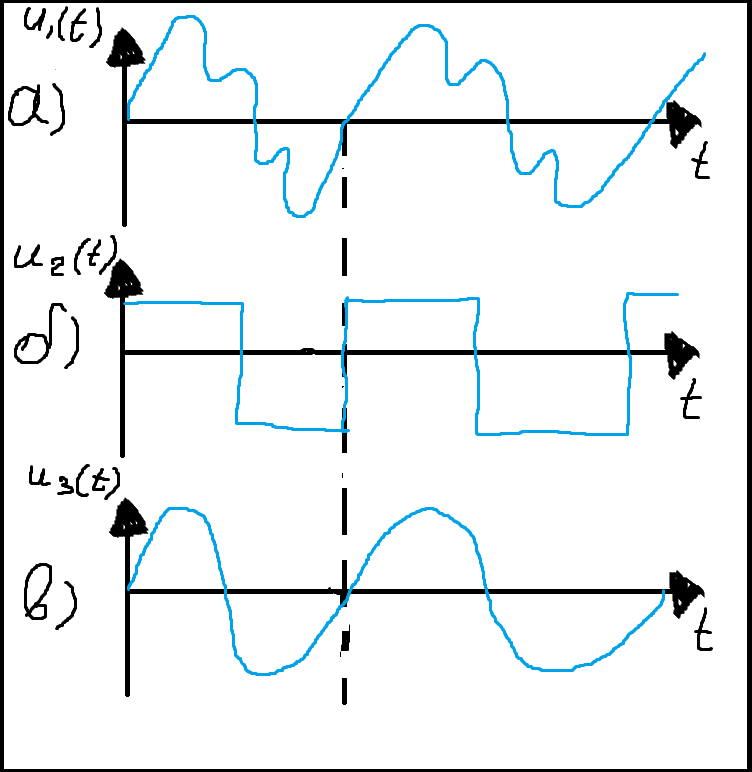
\includegraphics[width=6cm, height=6.2cm ]{images/pic1.png}\\
\floatsetup{Рис. 1}\\

\noindent колебания возникают только в одном контуре с собственной частотой $\nu_0$. Очевидно, для таких колебательных периодический процесс $u_3(t)$ является простейшим, поскольку он вызывает возбуждение только на одной частоте, равной $\nu_0$. Этот процесс вам, безусловно, знаком, он представляет собой так называемое синусоидальное, или гармоническое, колебание, описываемое соотношением \[u(t) = A\sin({2\pi\nu_0t + \phi}) = A\sin({\omega_0t + \phi}),\]\\

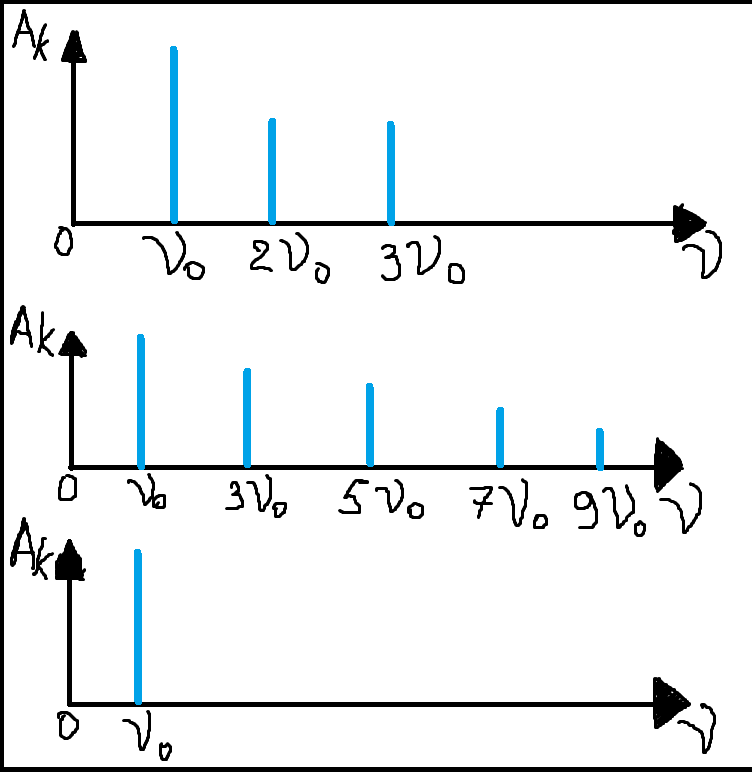
\includegraphics[width=6cm, height=6.2cm ]{images/pic2.png}\\
\floatsetup{Рис. 2}

\noindent и удовлетворяющее условиям \[ A, \omega_0, \phi = const \] где $A$ - амплитуда, $\phi$ - начальная фаза, $\omega_0 = 2\pi\nu_0$ - круговая частота колебаний. \par Как же объяснить тот факт, что каждый из сигналов $u_1(t)$ и $u_2(t)$ одновременно возбуждает несколько конутров, настроенных на разные частоты? Можно заметить, что эти  сигналы ведут себя так, как если бы каждый из них представлял собой сумму нескольких синусоидальных колебаний с разными частотами. Строго это свойство было доказано французским учёным Фурье и сформулировано им в виде замечательной теоремы. Она утверждает, что практически любую периодическую функцию, частота которой равна $\nu_0$, можно представить в виде суммы синусоид с соответсвующим образом подобранными амплитудами и начальными фазами и частотами, кратными $\nu_0$ (такие синусоиды часто называют гармоническими), или, как говорят, эту функцию можно разложить в ряд Фурье. Эта теорема может быть записана следующим образом:\\
$ u(t) = A_1\sin({\omega_0t + \phi_1})  + A_2\sin({2\omega_0t + \phi_2}) + A_3\sin({3\omega_0t + \phi_3}) + ... + A_k\sin({k\omega_0t + \phi_k}) + ...$\\

или, более кратко, \[u(t) = \sum_{k=1}^{\infty}A_k\sin({k\omega_0t + \phi_k})\] где $k$ - номер гармоники, определяяющий её частоту, $A_k$ - амплитуда гармоники, $\phi_k$ - начальная фаза гармоники, $\omega_0$ - круговая частота исследуемого процесса. \par Таким образом, сигнал представленный в виде суммы синусоид, можно удобно и просто охарактеризовать совокупностью величин $A_k$ и $\phi_k$. Совокупность величин $A_k$ называется спектром амплитуд. Этот спектр наглядно представляют графически, откладывая по оси ординат значения $A_k$ и по оси абсцисс $\nu$ и изображая амплитуды отдельных гармоник

\end{multicols}

\end{document}
